\documentclass[10pt]{myland}

%%%%%%%%%%%%%%%%%%%%%%%%%%%%FILE TITLE%%%%%%%%%%%%%%%%%%%%%%%%%%%%%%%%%%%%
\begin{document}
\begin{center}
	{\Large \myhwname{CSE 444: Lab 2 Writeup}} \\
	\vspace{.05in}
    \myname{Linxing Preston Jiang}\quad\quarter{Winter 2018}\\
	\vspace{.05in}
    \today \\
\end{center}
\vspace{.15in} \hrule \vspace{0.5em}%


\begin{enumerate}[label=\textbf{\arabic*.}, listparindent=0.0em, itemsep=1em]
    \item Query runtime
        \begin{itemize}
            \item Query 1: 1.53 seconds (\texttt{attu4})
            \item Query 2: Because of nested-loop-join implementation, Query 2 takes forever to finish (did not finish
                after an eight hour tmux session on \texttt{attu4})
            \item Query 3: Same as above
        \end{itemize}
	\item
	Lab 2 consists two major parts: operators \& aggregates, and database mutability. For the first part, we implemented
    \texttt{Filter}, \texttt{Join} operator and common aggregates such as \texttt{MIN, MAX, AVG}. For the second part,
    we focused on the implementation of inserting/deleting tuples to and from the database, also the eviction of pages
    in \texttt{BufferPool} when it's full. Key components implemented are:
	\begin{itemize}
        \item \texttt{Predicate}: this defines a predicate (comparision) which is needed for operators such as
            \texttt{Filter} and \texttt{Join} for tuple and field comparisons. \texttt{JoinPredicate} is designed directly
            for \texttt{Join} operation.
		\item \texttt{Join}: The class represents the join operation for relational database. The \texttt{Join} operator
            takes in tuples from two child iterator and use \texttt{JoinPredicate} to filter results.
		\item \texttt{Aggregate}: this represents an aggregation clause, can be on \texttt{Integer} or \texttt{String}
            fields. \texttt{Aggregate} loads all tuples from child at \texttt{open()} and returns the aggregate results
            one group at a time in \texttt{next()}.
		\item \texttt{HeapPage}: We added \texttt{insert}, \texttt{delete} in it, which insert/delete tuples to/from the
            \texttt{tuple} array and mark the corresponding slots to used/free. \texttt{HeapPage} directly inserts/deletes
            tuples to/from the \texttt{Tuple} array which will be the data updated on disk.
        \item \texttt{HeapFile}: We added \texttt{insert}, \texttt{delete} in it, which obtains the page from
            \texttt{BufferPool} (Or add a new empty page when added) and calls the \texttt{insert/delete} from
            \texttt{HeapPage}. Also, we added \texttt{writePage} method which is needed later for \texttt{BufferPool}
            to write the data on dirty \texttt{HeapPages} to disk.
		\item \texttt{BufferPool}: We added \texttt{insert}, \texttt{delete} in it, which insert/delete tuples to/from the
            pages in BufferPool by calling the method from \texttt{HeapFile} to update the page, then \texttt{BufferPool}
            updates the records by re-inserting the pages into the \texttt{BufferPool}. When the \texttt{BufferPool} is
            full and a new page need adding, \texttt{writePage} from \texttt{HeapFile} will be called to write the dirty
            page to disk and add the new page into the \texttt{BufferPool}. \texttt{BufferPool} is in charge of updating
            the pages because \texttt{Insert/Delete} operators directly call \texttt{insert/delete} of \texttt{BufferPool}.
	\end{itemize}
    \newpage
    \par Examples:
    \par Workflow (\texttt{join()}, showing \texttt{next()} call): \\
    \begin{center}
        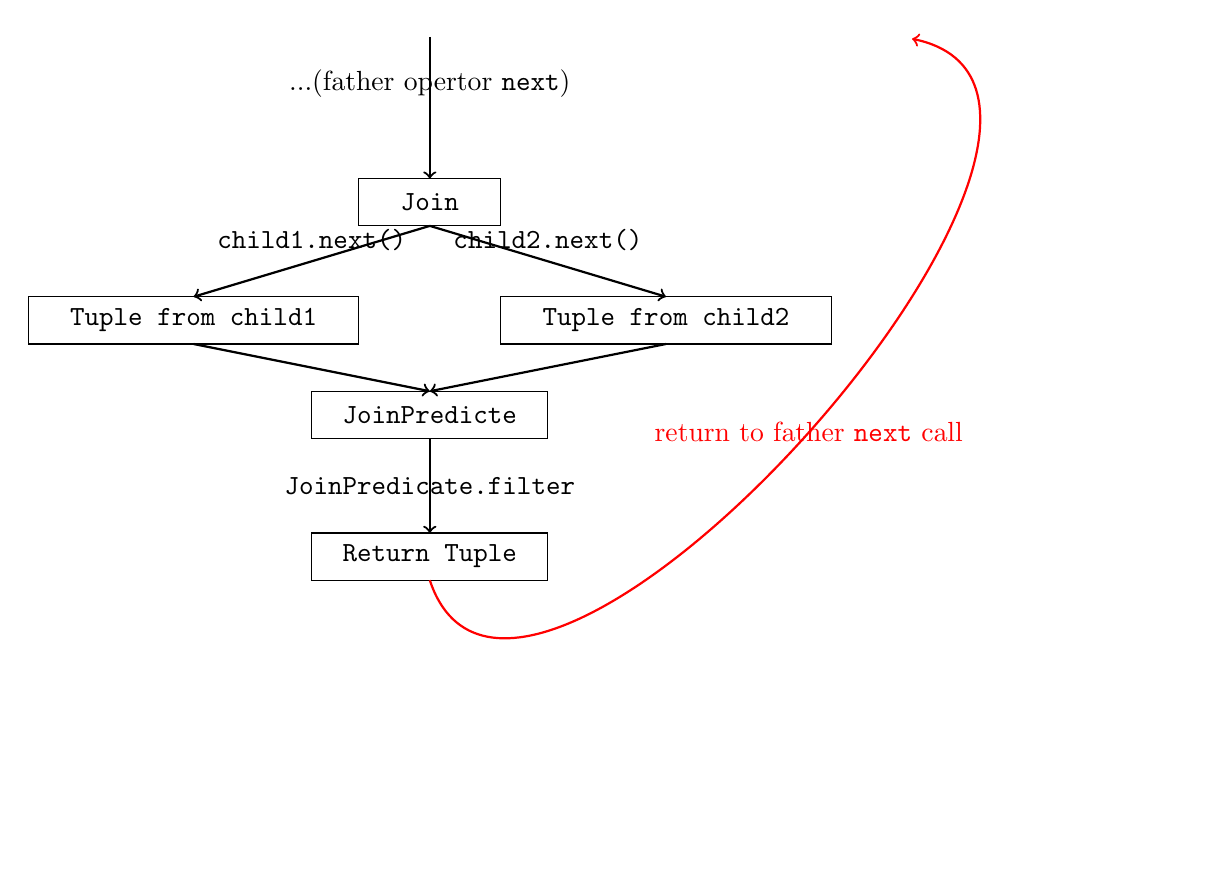
\begin{tikzpicture}[
            scale=.6,
        ]
            \path[->, thick] (0, 3) edge node[midway, above] {...(father opertor \texttt{next})} (0, 0);
            \draw[draw=black] (-1.5, 0) rectangle (1.5, -1) node[midway]  {\texttt{Join}};
            \path[->, thick] (0, -1) edge node[midway, above] {\texttt{child1.next()}} (-5, -2.5);
            \path[->, thick] (0, -1) edge node[midway, above] {\texttt{child2.next()}} (5, -2.5);
            \draw[draw=black] (-8.5, -2.5) rectangle (-1.5, -3.5) node[midway]  {\texttt{Tuple from \texttt{child1}}};
            \draw[draw=black] (1.5, -2.5) rectangle (8.5, -3.5) node[midway]  {\texttt{Tuple from \texttt{child2}}};
            \path[->, thick] (-5, -3.5) edge node[midway, above] {} (0, -4.5);
            \path[->, thick] (5, -3.5) edge node[midway, above] {} (0, -4.5);
            \draw[draw=black] (-2.5, -4.5) rectangle (2.5, -5.5) node[midway]  {\texttt{JoinPredicte}};
            \path[->, thick] (0, -5.5) edge node[midway] {\texttt{JoinPredicate.filter}} (0, -7.5);
            \draw[draw=black] (-2.5, -7.5) rectangle (2.5, -8.5) node[midway]  {\texttt{Return Tuple}};
            \node (father) at (10, 3) {};
            \path[->, thick, color=red] (0, -8.5) edge [bend right=120] node[midway] {return to father \texttt{next} call} (father);
        \end{tikzpicture}
    \end{center}
    Workflow (\texttt{insertTuple()}): \\
    \begin{center}
        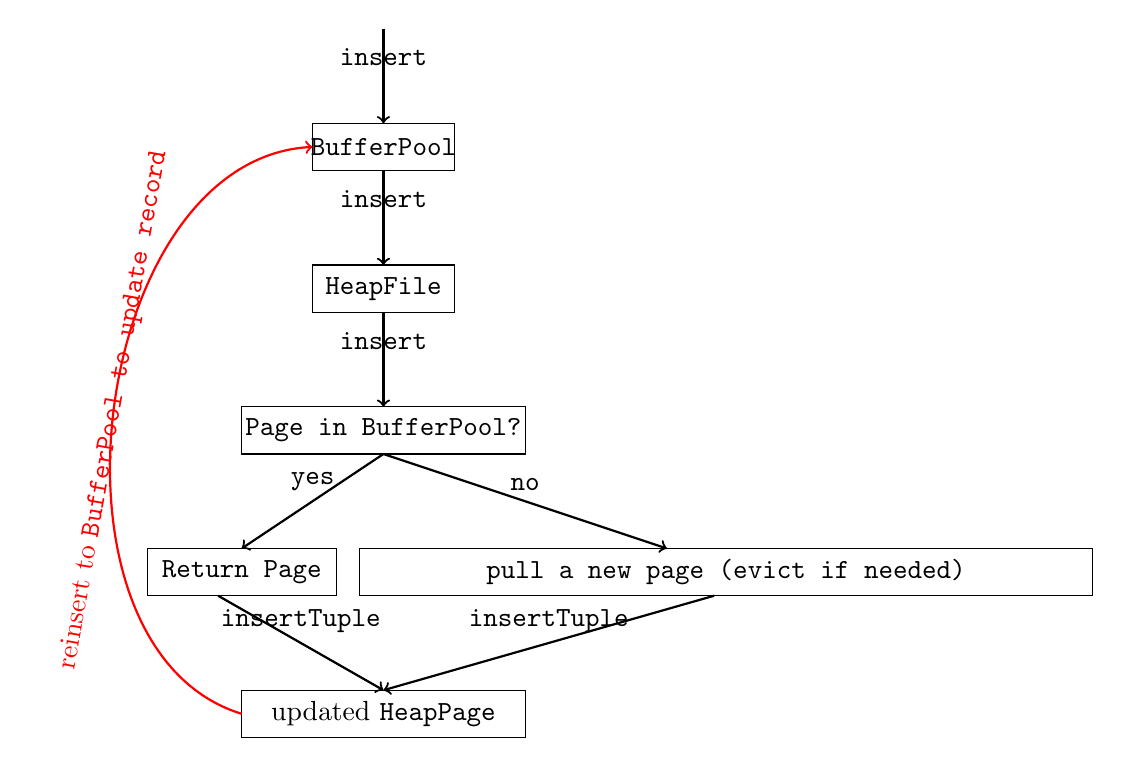
\begin{tikzpicture}[
            scale=.6,
        ]
            \path[->, thick] (0, 2) edge node[midway, above] {\texttt{insert}} (0, 0);
            \draw[draw=black] (-1.5, 0) rectangle (1.5, -1) node[midway]  {\texttt{BufferPool}};
            \path[->, thick] (0, -1) edge node[midway, above] {\texttt{insert}} (0, -3);
            \draw[draw=black] (-1.5, -3) rectangle (1.5, -4) node[midway]  {\texttt{HeapFile}};
            \path[->, thick] (0, -4) edge node[midway, above] {\texttt{insert}} (0, -6);
            \draw[draw=black] (-3, -6) rectangle (3, -7) node[midway]  {\texttt{Page in BufferPool?}};
            \path[->, thick] (0, -7) edge node[midway, above] {\texttt{yes}} (-3, -9);
            \path[->, thick] (0, -7) edge node[midway, above] {\texttt{no}} (6, -9);
            \draw[draw=black] (-5, -9) rectangle (-1, -10) node[midway]  {\texttt{Return Page}};
            \draw[draw=black] (-0.5, -9) rectangle (15, -10) node[midway]  {\texttt{pull a new page (evict if needed)}};
            \path[->, thick] (-3.5, -10) edge node[midway, above] {\texttt{insertTuple}} (0, -12);
            \path[->, thick] (7, -10) edge node[midway, above] {\texttt{insertTuple}} (0, -12);
            \draw[draw=black] (-3, -12) rectangle (3, -13) node[midway]  {updated \texttt{HeapPage}};
            \path[->, thick, color=red] (-3, -12.5) edge [bend left=80] node[midway, rotate=80] {reinsert to \texttt{BufferPool
                to update record}} (-1.5, -0.5);
        \end{tikzpicture}
    \end{center}
    \newpage

    \item Design decisions: I chose to use nested loop join. Nested-loop-join is the slowest but it works for all kinds
        of comparisons (Hash join only works well for equality comparison, sort-merge join only works well for inequaliy
        comparison). For eviction policy, I chose to evict the first page every time the \texttt{BufferPool} is full.
        This does not work well in terms of keeping most commonly used page in memory, which result in extra disk IOs,
        but the implementation is easy and does not require extra data structures in order to keep track of page usage.

    \item Extra Unit tests: A unit test for the correctness of HeapFile insertTuple behavior would be great. The spec
        requires the update of \texttt{BufferPool} pages to happen in the insert/delete methods of \texttt{BufferPool}
        instead of in \texttt{HeapFile}. I did it the wrong way and caused the \texttt{handleManyDirty} test to fail, and
        it took me a while to realize that test uses a overriden \texttt{insert} method and \texttt{BufferPool} should
        be in charge of updating the record.

    \item Changes to API: I did not make changes to the APIs given.

    \item Missing elements: I believe I finished the entire Lab 2
\end{enumerate}
\end{document}
